\chapter{Background}\label{back}

\lettrine{I}{}\textit{n} this Chapter, we explain the main concepts and used tools related to Agora. This work has been thought for HPC applications that run in parallel architectures, so we start clarifying what are these target systems and how they are built. After that, we explain the concepts of Design Space Exploration and Design of Experiments, that represents the kernel of this work, together with the idea of application dynamic online autotuning. Finally, we present the tools used for communications among Agora components and for application complete model prediction, highlighting their principal characteristics and features: the Message Queue Telemetry Transport (MQTT) messaging protocol and the Generalized Linear Regression interface by Apache Spark\textsuperscript{TM} Machine Learning MLlib library.

\section{Target architecture}

High Performance Computing applications have complex and massive tasks to do, so they need huge computing power in order to accomplish their objectives.

Parallel computing (\cite{barney2012introduction}) simultaneously uses multiple re\-sourc\-es in order to solve a computational problem, taking advantage of concurrency, that is the possibility to execute, at the same time, those parts that are independent each other. In figure \ref{fig::pC::serial} we can see an example of serial computation, with a single processor that executes problem instructions sequentially, one after another. Figure \ref{fig::pC::parallel} instead represents a possible parallel computation, where problem is split in four parts that can be executed concurrently on different processors.

\begin{figure}[htb]

    \centering

    \subfloat[][\emph{Serial computation}\label{fig::pC::serial}]
        {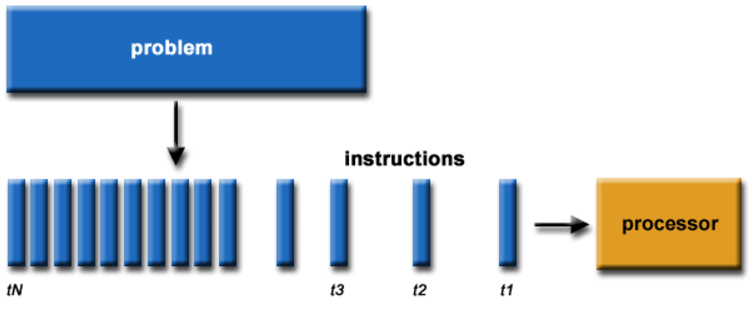
\includegraphics[width = 0.49\textwidth]{ser_prob}}
    \enskip
    \subfloat[][\emph{Parallel computation}\label{fig::pC::parallel}]
        {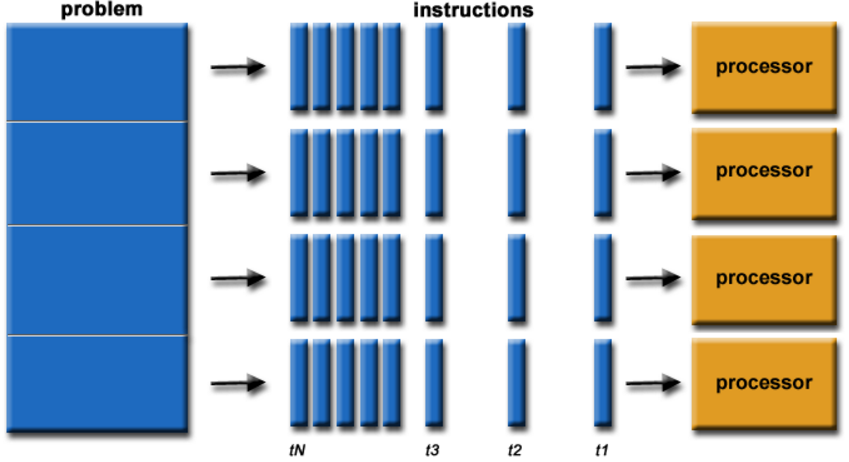
\includegraphics[width = 0.49\textwidth]{par_prob}}
    
    \caption{Serial and parallel computation of a problem}

\end{figure}

A typical parallel architecture is composed by an arbitrary number of computers, called \textit{nodes}, each of them with multiple processors, cores, functional units, ect. connected all together by a network.

\begin{figure}[htb]

    \centering
    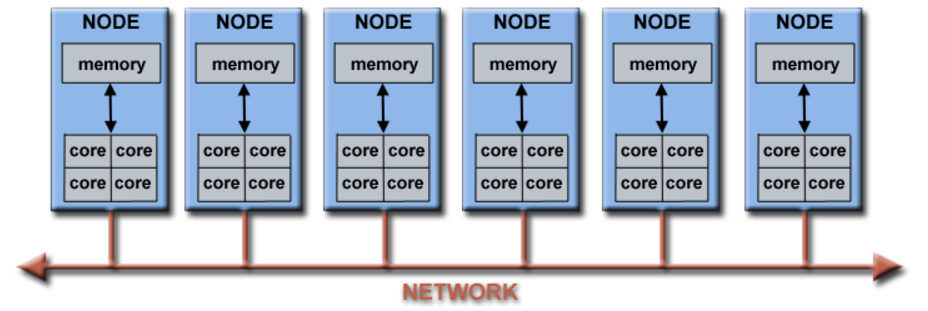
\includegraphics[width = \textwidth]{par_net}
    \caption{Parallel architecture schema}

\end{figure}

Inside a parallel architecture there can be heterogeneous nodes, with different computing techniques and configurations; according to Flynn's classical taxonomy, we can identify four different ways to classify computing architectures: 

\begin{enumerate}

    \item \textit{Single Instruction, Single Data (SISD)}: this is the original kind of computer, in which there is only one instruction stream that is managed by the Central Processing Unit (CPU) during clock cycles. This is serial, so non-parallel, computing;
    
    \item \textit{Single Instruction, Multiple Data (SIMD)}: at any clock cycle, there is one instruction that is executed, but processing units can operate on different data elements of instruction;
    
    \item \textit{Multiple Instruction, Single Data (MISD)}: a single data stream is managed by multiple processing units, that can independently operate on data through separate instruction streams;
    
    \item \textit{Multiple Instruction, Multiple Data (MIMD)}: every processing unit can execute different data and instruction streams.

\end{enumerate}

Nowadays, among introduced alternatives, MIMD architectures are the most used in parallel computing, especially in HPC systems.





\section{Design Space Exploration}

In many engineering problems there are several objectives that have to be obtained, given certain constraints and with the possibility to manage some customizable parameters. Objectives can involve various metrics of interest, for instance connected to application throughput, system consumed power or overall cost.

Automatic Design Space Exploration (DSE) analyzes, in a systematic way, the space of possible parameter combinations that constitute application Design Space, with the objective to find the best design point that fulfills problem goals and requirements.

HPC applications have almost always a lot of parameters and related set of values, making the list of program configurations very long. In these cases, the corresponding Design Space literally explodes, making impossible to analyze it in an exhaustive way.

\subsection{Multi-Objective Optimization (MOO) problem}

When there is more than one objective function, DSE consists of a Multi-Objective Optimization (MOO) problem. Taking \cite{caramia2008multi} as reference, in mathematical terms a MOO problem can be defined as:

\begin{equation}
        min( f_1(x), f_2(x), ..., f_k(x) ), \quad k \ge 2 \qquad s.t. \quad x \in X
\end{equation}

where $k$ denotes the number of objective functions and $X$ represents the feasible region, defined by some constraints functions (for instance, in an embedded architecture, the total area should not exceed a predetermined value). If some of the objective functions have to be maximized, they can be attributed to minimizing its negation.

Multi-Objective Optimization problem has a lot of analogies into a wide variety of situations and domains, even the most common ones. Formerly the ancients, given a set of seeds and a plot of land, had to choose what, how and how much farm, in order to maximize harvest profit and to minimize required effort, simultaneously not exceeding a cost limit. Airline companies want to augment the number of passengers on their airplanes, to increase safety, to enlarge autonomy of their vehicles by means of various technical, strategic and commercial choices. An undergraduate student would minimize his/her university career duration and maximize his/her exam average, with a predetermined time limit and with the possibility to choose some coursers than others.

Since some objectives are in contrast with other objectives, a unique solution does not exist. For instance, in a microcontroller, an objective focused on performance would definitely confront against a goal related to power consumption: best solution for one of them would be the worst for the other and conversely. Therefore, the aim of Design Space Exploration is almost always to search for a trade off, among goals and requirements, that fulfills overall problem.

Since the concept of unique optimal solution can't be applied, it is useful to introduce the notion of Pareto optimality. Pareto optimal solutions are, essentially, those ones that can't be improved without degrading at least one objective function. So, a solution \textit{x\textsuperscript{1}} is said to \textit{(Pareto) dominate} a solution \textit{x\textsuperscript{2}} if:

\begin{equation}
\begin{cases}
        f_i(x^1) \le f_i(x^2) \quad \forall i \in \{1, 2, ..., k\} \\
        f_j(x^1) < f_j(x^2) \quad \textit{for at least one } j \in \{1, 2, ..., k\}
\end{cases}
\end{equation}

The set of Pareto optimal solutions is often called Pareto front, Pareto frontier or Pareto boundary.





\section{Design of Experiments}\label{doe}

When a Design Space of an application is huge and, consequently, there is no possibility to do an exhaustive analysis of all possible configurations, there is the need to take a subset of points of interest that represent as closely as possible system behavior. Therefore, on one hand there is the quality of representation, that should be reliable enough; on the other side, the number of simulations to do, that should be small.

Taking \cite{natrella2013nist} as reference, among various DoE techniques that generate initial set of design points to be analyzed, we can mention:

\begin{itemize}

    \item \textit{Full-Factorial DoE}: it is given by all possible combinations among parameter values, so all possible application configurations are picked up;
 
    \item \textit{2-Level Full-Factorial DoE}: suitable for designs with two or more parameters, this DoE picks up all possible combinations among the extreme values of all parameters.
    
    If, for instance, there are three tunable parameters:
    
    \begin{enumerate}
    
        \item Number of Processors $\in$ \{ 2, 4, 8, 16, 32 \};
        
        \item Number of Threads $\in$ \{ 1, 2, 3, 4, 5, 6, 7, 8 \};
        
        \item Cache size $\in$ \{ 2K, 4K, 8K, 16K, 32K \}.
    
    \end{enumerate}
    
    design points will be: \hbox{$\langle$ \#processors, \#threads, cache size $\rangle$} $\in$
    
    \{ $\langle$ 2, 1, 2K $\rangle$, $\langle$ 32, 1, 2K $\rangle$, $\langle$ 2, 8, 2K $\rangle$, $\langle$ 32, 8, 2K $\rangle$, \hbox{$\langle$ 2, 1, 32K $\rangle$}, \hbox{$\langle$ 32, 1, 32K $\rangle$}, $\langle$ 2, 8, 32K $\rangle$, $\langle$ 32, 8, 32K $\rangle$ \};

    \item \textit{Face Centered Central Composite DoE with one Center Point}: also this DoE is appropriate for designs with two or more parameters. Design point list can be split in three sets:
    
     \begin{enumerate}
    
        \item A 2-Level Full-Factorial Design set;
        
        \item A Center Point, in which each value is the median value of corresponding parameter;
        
        \item An Axial Point set, in which all median and extreme values of each parameter are combined.
    
    \end{enumerate}
    
    Considering the example in previous DoE, final design point list would be: $\langle$ \#processors, \#threads, cache size $\rangle$ $\in$
    
    \{ $\langle$ 2, 1, 2K $\rangle$, $\langle$ 32, 1, 2K $\rangle$, $\langle$ 2, 8, 2K $\rangle$, $\langle$ 32, 8, 2K $\rangle$, \hbox{$\langle$ 2, 1, 32K $\rangle$}, \hbox{$\langle$ 32, 1, 32K $\rangle$}, $\langle$ 2, 8, 32K $\rangle$, $\langle$ 32, 8, 32K $\rangle$ \} $\cup$ 
    
    \{ $\langle$ 8, 4, 8K $\rangle$ \} $\cup$
    
    \{ $\langle$ 2, 4, 8K $\rangle$, $\langle$ 32, 4, 8K $\rangle$, $\langle$ 8, 1, 8K $\rangle$, $\langle$ 8, 8, 8K $\rangle$, $\langle$ 8, 4, 2K $\rangle$, \hbox{$\langle$ 8, 4, 32K $\rangle$} \};
    
    \item \textit{Plackett-Burman DoE}: it might be useful to analyze, more eonomically, a larger number of parameters. This DoE reduces the number of potential factors, constructing very economical designs with number of points multiple of 4 (rather than power of 2, as in the 2-Level Full-Factorial DoE).
    
    Concerning the example above, in this case final design point list would be: $\langle$ \#processors, \#threads, cache size $\rangle$ $\in$
    
    \{ $\langle$ 2, 1, 32K $\rangle$, $\langle$ 32, 1, 2K $\rangle$, $\langle$ 2, 8, 2K $\rangle$, $\langle$ 32, 8, 32K $\rangle$ \};
    
    \item \textit{Latin-Hypercube DoE}: this DoE randomly chooses parameter values for each design point. The number of final configurations can be set up in advance.

\end{itemize}





\section{Dynamic Autotuning}

When applications expose some configurable parameters (a.k.a. \textit{dynamic knobs}), the concept of Dynamic Autotuning is defined as the capability to find the best set of knob values, in an automatic and systematic way, that satisfies application goals and requirements at runtime, properly reacting to possible objective function change. For instance, a web video streaming application would be able to manage video quality according to the overload of its servers. In some situations, it could set up itself for the best possible resolution. Sometimes, it should reduce the quality in order to make still available its services to all connected clients.

IBM research studies on \textit{Autonomic Computing} (\cite{kephart2003vision}, \cite{computing2006architectural}) made a breakthrough on the concept of self-adapting systems that are able to manage themselves and to dynamically optimize their execution configuration at runtime. \textit{Autonomic Computing} is based of the MAPE-K control loop, showed in Figure \ref{fig::mape-k}.

\begin{figure}[htb]

    \centering
    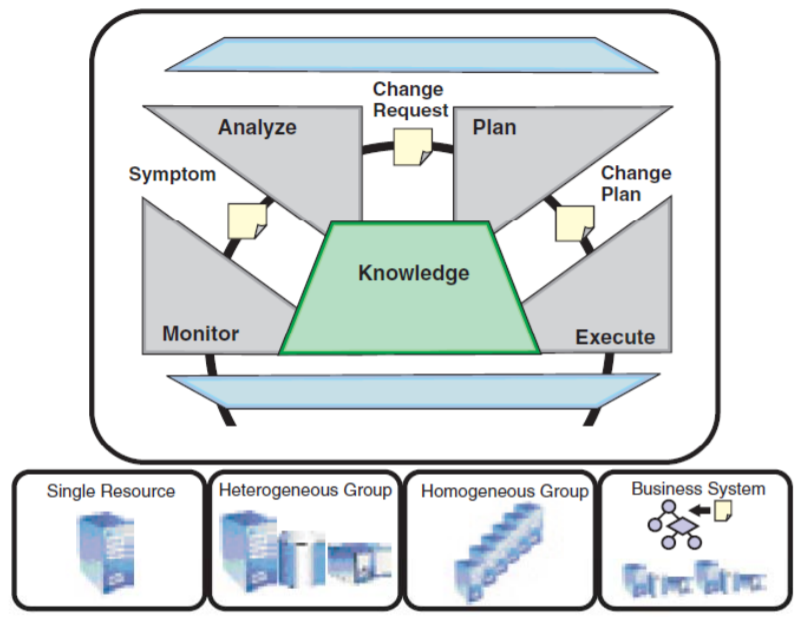
\includegraphics[width = \textwidth]{MAPE-K}
    \caption{MAPE-K control loop design}
    \label{fig::mape-k}

\end{figure}

In this control loop we can identify four principal functions:

\begin{itemize}

    \item \textit{Monitor}: it gathers application information about knob setting and associated metric of interest values as, for instance, throughput and consumed power;
    
    \item \textit{Analyze}: it performs data analysis and reasoning on information provided by the monitor function;
    
    \item \textit{Plan}: it reacts to a possible application objective change during execution and it structures the actions needed to achieve this new state;
    
    \item \textit{Execute}: it modifies the behavior of managed resource, according to actions recommended by the plan function.

\end{itemize}

Finally, \textit{Knowledge} source is composed of all data that is used by the four functions; it includes information such as, for instance, topology structure, historical logs, metrics and policies.

Online autotuning, therefore, entrusts system management from people to technology, achieving self-configuration and self-op\-ti\-mi\-za\-tion objectives. Application requirements may change during execution and the overall system is able to properly react and to re-adapt itself.





\section{MQTT messaging protocol}\label{mqtt}

MQTT (Message Queue Telemetry Transport, \cite{banks2014mqtt}) is a light\-weight messaging protocol that gives the possibility to establish remote communications among subjects. Its main characteristics are the minimization of network bandwidth and devices requirements. This features make MQTT ideal for machine-to-machine (M2M) or Internet of Things (IoT) world of connected devices, but in general this protocol have a large use in different projects; for instance, famous Facebook Messenger is built on top of it (\cite{zhang2011building}).

MQTT uses a client server publish\slash{}subscribe pattern. A client has the possibility to subscribe to topics and to publish messages on them (both topics and messages are strings). Another component, called \textit{broker} server, deals with the dispatch of messages to only clients that have subscribed to corresponding topic. Therefore, publishers (clients that sends messages) and subscribers (clients that receive messages) don't know about the existence of one another: the broker, which is known by every client, distribute messages accordingly. Figure \ref{fig::mqtt_example} shows a possible MQTT scenario with a sensor and two devices.

\begin{figure}[htb]

    \centering
    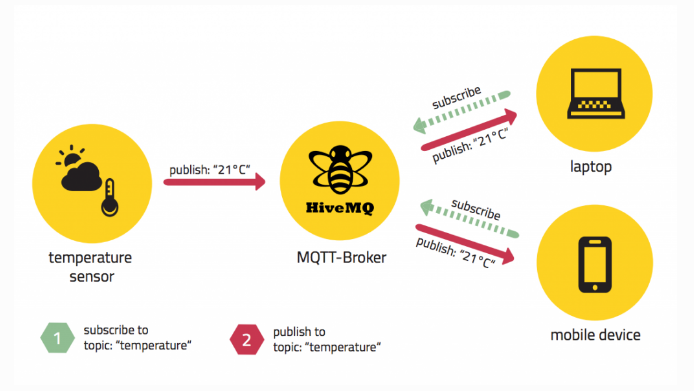
\includegraphics[width = \textwidth]{mqtt}
    \caption{MQTT publish/subscribe example, taken from \cite{site:hivemq}}
    \label{fig::mqtt_example}

\end{figure}

Topics are used by the broker to filter messages and to manage them in a correct way; they are made up of one or more levels, separated by a forward slash, as shown in Figure \ref{fig::topic}.

\begin{figure}[hb]

    \centering
    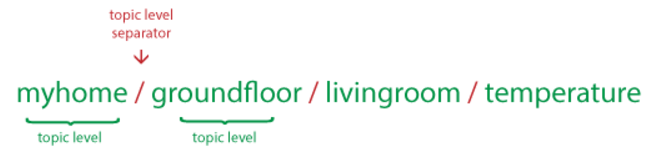
\includegraphics[width = \textwidth]{mqtt_toplevs}
    \caption{A MQTT topic, taken from \cite{site:hivemq}}
    \label{fig::topic}

\end{figure}

There is the possibility to subscribe to more topics at once through the use of wildcards: the single-level one (denoted with the symbol \textit{+}) and the multi-level one (indicated with the symbol \textit{\#}).

Single-level wildcard substitutes an arbitrary level in a topic, so all topics that matches the same structure are associated to the one with single-level wildcard.
For instance,\\
\centerline{\textit{myhome\slash{}groundfloor\slash{}kitchen\slash{}temperature}}\\
\centerline{and}\\
\centerline{\textit{myhome\slash{}groundfloor\slash{}livingroom\slash{}temperature}}\\
match topic in Figure \ref{fig:mqtt_singlew}, while\\
\centerline{\textit{myhome\slash{}groundfloor\slash{}kitchen\slash{}humidity}}\\
don't.

\begin{figure}[htb]

    \centering
    
\includegraphics[width = 0.8\textwidth]{mqtt_singlew}
    \caption{A MQTT topic with single-level wildcard, taken from \cite{site:hivemq}}
    \label{fig:mqtt_singlew}

\end{figure}

Multi-level wildcard is placed at the end of a topic and it covers an arbitrary number of topic levels.
In this case, for instance,\\
\centerline{\textit{myhome\slash{}groundfloor\slash{}kitchen\slash{}tem\-per\-a\-ture}}\\
\centerline{and}\\
\centerline{\textit{myhome\slash{}groundfloor\slash{}kitchen\slash{}humidity}}\\
match topic in Figure \ref{fig:mqtt_mulw}, while\\
\centerline{\textit{myhome\slash{}firstfloor\slash{}livingroom\slash{}temperature}}\\
don't.

\begin{figure}[htb]

    \centering
    
\includegraphics[width = 0.8\textwidth]{mqtt_mulw}
    \caption{A MQTT topic with multi-level wildcard, taken from \cite{site:hivemq}}
    \label{fig:mqtt_mulw}

\end{figure}

Another interesting MQTT feature is the Last Will and Testament (LWT). Each client can specify a normal MQTT message with topic and payload. When it connects to the broker, this message is stored; if client abruptly disconnects, broker sends corresponding LWT to all subscribed clients on related topic, notifying occurred disconnection.





\section{Apache Spark\texorpdfstring{$^{TM}\;$}MMLlib library}

Agora takes advantage of the Machine Learning MLlib library by Apache Spark\textsuperscript{TM} (\cite{spark2015apache}) in order to predict complete model of running applications; in particular, we focuse on the Generalized Linear Regression interface.


\subsection{(Generalized) Linear Regression}\label{glr}

Taking \cite{site:caltechML2012} as reference, Linear Regression tries to model the relationship between a variable $y$ and one or more variables $x_1,x_2,...x_n,n\ge1$. More rigorously, given a set of statistical units $\{y_i,x_{i1},x_{i2},...,x_{ip}\}_{i = 1}^n$, in which $y_i$ is the variable that depends on the p-vector $[x_{i1}, x_{i2}, ..., x_{ip}]$, linear regression assumes that this relationship is linear:

\begin{equation}
    y_i = \beta_0\boldsymbol{1} + \beta_1x_{i1} + \beta_2x_{i2} + ... +  \beta_px_{ip} + \epsilon_i, \quad i = 1, 2, ... n
\end{equation}

$y_i$ is the \textit{response variable} or \textit{regressand};

$x_{i1}, x_{i2}, ..., x_{ip}$ are called \textit{independent variables} or \textit{regressors};

$\beta_0, \beta_1, ..., \beta_p$ are the \textit{regression coefficients}, whose values establish the relationship among regressand and regressors; $\beta_0$ is also called \textit{intercept}. Linear regression mainly focuses on the estimation of these parameters;

$\epsilon_i$ is called the \textit{error term}. It represents all other factors that influence $y_i$ other than the independent variables.

Linear Regression assumes that the response variable follows a Gaussian distribution. Generalized Linear Regression (GLR) gives the possibility to specify other distributions taken from the exponential family. It is useful for several kinds of prediction problems, including Linear Regression, Poisson Regression (for count data) and Logistic Regression (for binary data). Moreover, GLR gives the possibility to specify the link function \textit{g} that relates the mean of regressand to the independent variables. In case of Gaussian distribution for Linear Regression, the link function can be equal to \textit{Identity}, \textit{Log} and \textit{Inverse}, with explicit meaning.


\subsection{Regressor transformations}\label{regrTransforms}

In order to use Linear Regression even if the relationship among response variable and independent variables is not linear, there is the necessity to modify input variables. Agora implements two possible independent variable transformations:

\begin{enumerate}

    \item it transforms parameter values with inverse, square root and natural logarithmic functions. In union with the unaltered predictor variables, it tries to find the best model combining these transformations and available link functions. We refer to this strategy as \textit{"transformations by functions"};
    
    \item it transforms parameter values through polynomial combinations of degree 2: their cross-products and square values are added to the set of regressors, evaluating the best model with available link functions. We refer to this strategy as \textit{"polynomial combinations of degree 2"}.

\end{enumerate}

Agora chooses the model with the smallest Akaike Information Criterion (AIC) value, that is a measure of the quality, in terms of lost information, of statistical models for a given set of data. At the same AIC value, chosen model is the one with the smallest mean of the sum of coefficient standard errors, that measure how precisely predicted model has estimated regression coefficients with the given training set of data.
